% !TEX root = ../termpaper.tex
% first example section
% @author Thomas Lehmann
%

\section{Einleitung}
In dieser Arbeit untersuchen wir einen Graphen mit n Knoten, bei dem jeder Knoten mit einer Wahrscheinlichkeit p mit jedem anderen Knoten verbunden ist. Zu Beginn wird für beliebige Werte von p und 
n die minimale Distanz zwischen allen Knotenpaaren ermittelt und eine statistische Auswertung vorgenommen. Im Anschluss erfolgt eine Analyse der Erwartungen, wie sich die statistischen Ergebnisse in Abhängigkeit von verschiedenen Werten für p und n darstellen. Schließlich werden die Ergebnisse visualisiert und interpretiert.


\section{Mein Ansatz und Vorüberlegungen}

Die statistische Analyse der minimalen Distanzen zwischen Knotenpaaren ist nur dann vollständig aussagekräftig, wenn der betrachtete Graph zusammenhängend ist. Da der Graph jedoch zufällig generiert wird und Knotenpaare nur mit der Wahrscheinlichkeit \( p \) verbunden sind, kann es vorkommen, dass er in mehrere unverbundene Komponenten zerfällt. In solchen Fällen wäre es sinnvoll, die statistische Auswertung für jede zusammenhängende Komponente separat durchzuführen, da zwischen Knoten in unterschiedlichen Komponenten keine Distanz existiert.

Da jedoch keine explizite Anforderung für die Anzahl der Komponenten gegeben ist, werde ich den Graphen so generieren, dass er als Ganzes zusammenhängend ist und somit eine globale statistische Auswertung ermöglicht. Dazu habe ich mir folgende Ansätze überlegt:

\begin{itemize}
    \item Ein iterativer Ansatz besteht darin, den Graphen zu erzeugen und anschließend zu überprüfen, ob er zusammenhängend ist. Falls dies nicht der Fall ist, wird ein neuer Graph generiert, bis ein zusammenhängender Graph erreicht wird.
    \item Alternativ kann die Wahrscheinlichkeit \( p \) erhöht werden, um die Chance auf einen zusammenhängenden Graphen zu steigern. Dies bietet jedoch keine absolute Garantie für Zusammenhängendheit. Ebenso erhöht eine größere Anzahl an Knoten die Wahrscheinlichkeit für einen zusammenhängenden Graphen, bleibt jedoch ebenfalls ohne Garantie.
\end{itemize}

In diesem Experiment werde ich den iterativen Ansatz verwenden, da er sicherstellt, dass der generierte Graph zusammenhängend ist.

\subsection{Erwartungen}

Für dieses Experiment erwarte ich folgende Beobachtungen:

\begin{itemize}
    \item Bei einer niedrigen Wahrscheinlichkeit \( p \) (unter 1\%) wird die Wahrscheinlichkeit eines zusammenhängenden Graphen sehr gering sein.
    \item Bei konstantem \( n \) und zunehmendem \( p \): Der Mittelwert der Distanzen wird gegen \( 1 \) konvergieren, und die Standardabweichung wird abnehmen.
    \item Bei konstantem \( p \) und zunehmendem \( n \): Der Mittelwert der Distanzen wird sinken, und die Standardabweichung wird tendenziell sinken.
\end{itemize}

\section{Versuchsaufbau und Durchführung}
Wir generieren Zufallsgraphen $G(n, p)$ mit $n$ Knoten und variieren die Wahrscheinlichkeit $p$. Für jede Kombination von $n$ und $p$ werden folgende Schritte durchgeführt:
\begin{enumerate}
    \item Der Graph wird mit der Wahrscheinlichkeit $p$ generiert und auf Zusammenhängendheit geprüft. Falls der Graph nicht zusammenhängend ist, wird der Graph neu generiert, bis er zusammenhängend ist.
    \item Für alle Knotenpaare wird die minimale Distanz berechnet.
    \item Die Ergebnisse werden statistisch ausgewertet. Dabei werden Mittelwert, Standardabweichung, Median und Quartile der Distanzen berechnet.
\end{enumerate}

Die verwendeten Wertebereiche für $n$ und $p$ sind wie folgt:
\begin{itemize}
    \item Anzahl der Knoten $n$: 100 bis 1000 in Schritten von 100.
    \item Verbindungswahrscheinlichkeit $p$: 0.1 bis 0.9 in Schritten von 0.1.
\end{itemize}

\section{Ergebnisse und Visualisierung}

\subsection{Mittelwerte der Distanzen}
In Abbildung \ref{fig:mean_distances} ist der Mittelwert der Distanzen für verschiedene Werte von $p$ und $n$ dargestellt. Hier zeigt sich, dass der Mittelwert der Distanzen sinkt, wenn $p$ größer wird, da mehr Verbindungen bestehen und kürzere Wege möglich sind. Bei hohen Werten von $p$ ist der Graph nahezu vollständig verbunden und die durchschnittliche Distanz nähert sich 1 an.

\begin{figure}
    \centering
    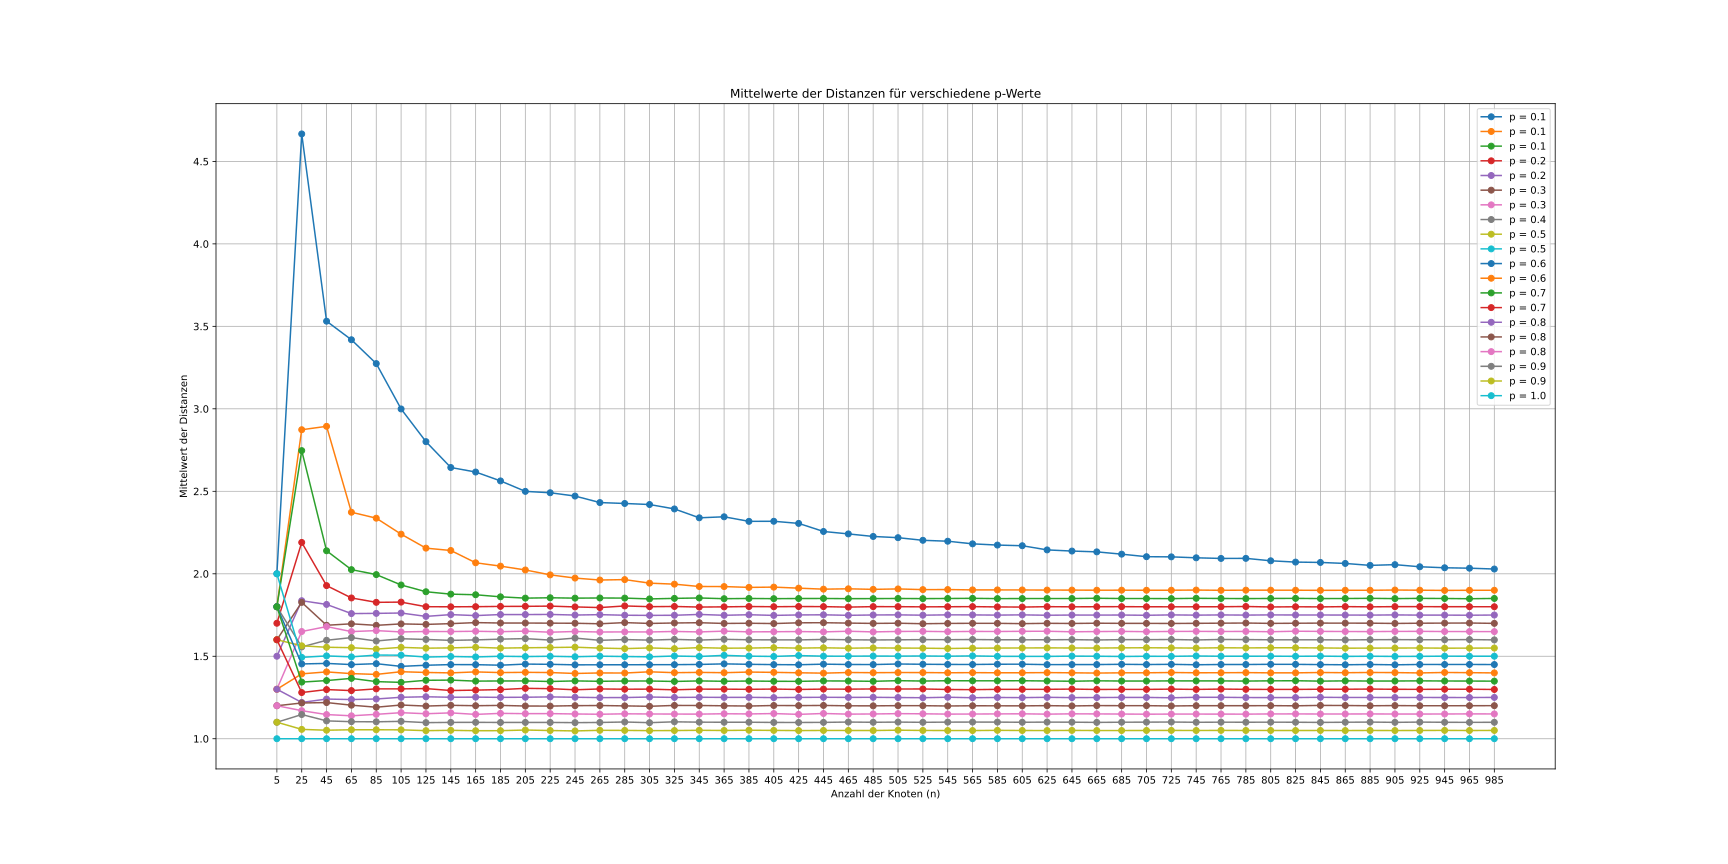
\includegraphics[width=\textwidth]{MittelwerteDistanzen}
    \caption{Mittelwerte der Distanzen für verschiedene $p$-Werte}
    \label{fig:mean_distances}
\end{figure}

\subsection{Standardabweichung der Distanzen}
In Abbildung \ref{fig:std_distances} ist die Standardabweichung der Distanzen für verschiedene Werte von $p$ und $n$ dargestellt. Es zeigt sich, dass die Standardabweichung bei kleineren $p$-Werten höher ist, da die Distanzen stärker variieren. Mit steigendem $p$ verringert sich die Standardabweichung, da die Distanzen homogener werden und kürzere Wege häufiger vorkommen.

\begin{figure}
    \centering
    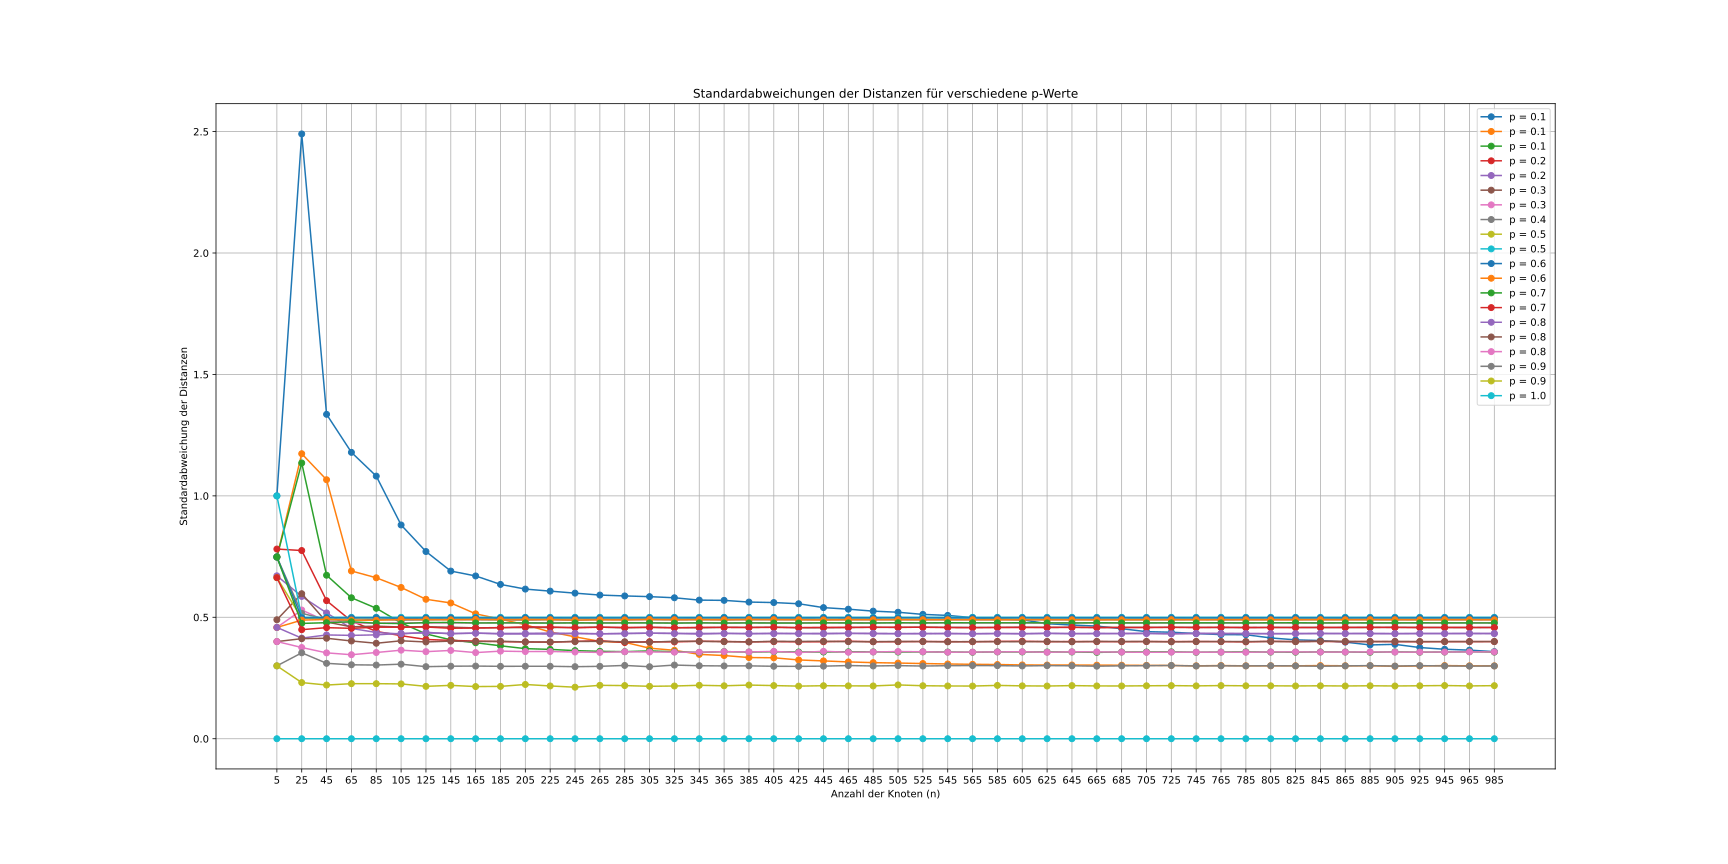
\includegraphics[width=\textwidth]{Standardabweichungen}
    \caption{Standardabweichungen der Distanzen für verschiedene $p$-Werte}
    \label{fig:std_distances}
\end{figure}

\section{Interpretation der Ergebnisse}
Die Ergebnisse bestätigen weitgehend unsere Erwartungen:
\begin{itemize}
    \item Für kleine Werte von $p$ ist der Graph oft nicht zusammenhängend. Erst ab einem bestimmten Schwellenwert (z.B. $p \approx 0.5$ bei $n = 100$) wird der Graph konsistent zusammenhängend.
    \item Mit steigendem $p$ sinken sowohl der Mittelwert als auch die Standardabweichung der Distanzen, da die Wahrscheinlichkeit für kürzere Verbindungen steigt und der Graph dichter wird.
    \item Bei konstantem $p$ und zunehmendem $n$ steigen die Distanzen zunächst, da es mehr Knoten gibt, zwischen denen die Distanz gemessen werden muss. Ab einer bestimmten Größe nehmen die Distanzen jedoch wieder ab, da sich die Struktur des Graphen durch zusätzliche Verbindungen stabilisiert.
\end{itemize}

Die Ergebnisse decken sich mit unserer Erwartung, dass ein dichterer Graph (höheres $p$) eine geringere durchschnittliche Distanz aufweist und die Abstände homogener verteilt sind.

\section{Fazit}
In diesem Experiment konnten wir die Auswirkung der Verbindungswahrscheinlichkeit $p$ und der Knotenzahl $n$ auf die minimalen Distanzen in einem zufällig generierten Graphen analysieren. Die Ergebnisse zeigen, dass mit zunehmender Dichte (größerem $p$) die durchschnittliche Distanz und die Streuung der Distanzen abnehmen. Zukünftige Experimente könnten die Analyse auf größere Graphen und andere Graphentypen ausweiten, um zu prüfen, ob ähnliche Muster beobachtet werden.

\end{document}